\documentclass[journal]{IEEEtran}
\ifCLASSINFOpdf
  \usepackage[pdftex]{graphicx}  
\else
\fi

% correct bad hyphenation here
\hyphenation{op-tical net-works semi-conduc-tor}
\usepackage[colorlinks=true]{hyperref}
\usepackage{amssymb}
\usepackage{algorithm}
\usepackage{amsmath}
\let\proof\relax
\let\endproof\relax
\usepackage{amsthm}
\usepackage{graphicx}
\usepackage{subfigure}
\usepackage{tabularx}
\usepackage{booktabs}
\usepackage{url}
\usepackage{bbm}
\usepackage[noend]{algpseudocode}
\usepackage{array}
\usepackage{balance}
\usepackage{multirow}
\usepackage{multicol}
\usepackage{threeparttable}
%\usepackage{cite}
\usepackage{subfigure}
\allowdisplaybreaks
\newcommand\algotext[1]{\end{algorithmic}#1\begin{algorithmic}[1]}


\newcommand{\var}{{\rm var}}
\newcommand{\Tr}{^{\top}}
\newcommand{\vtrans}[2]{{#1}^{(#2)}}
\newcommand{\kron}{\otimes}
\newcommand{\schur}[2]{({#1} | {#2})}
\newcommand{\schurdet}[2]{\left| ({#1} | {#2}) \right|}
\newcommand{\had}{\circ}
\newcommand{\diag}{{\rm diag}}
\newcommand{\invdiag}{\diag^{-1}}
\newcommand{\rank}{{\rm rank}}
\newcommand{\expt}[1]{\langle #1 \rangle}
% careful: ``null'' is already a latex command
\newcommand{\nullsp}{{\rm null}}
\newcommand{\tr}{{\rm tr}}
\renewcommand{\vec}{{\rm vec}}
\newcommand{\vech}{{\rm vech}}
\renewcommand{\det}[1]{\left| #1 \right|}
\newcommand{\pdet}[1]{\left| #1 \right|_{+}}
\newcommand{\pinv}[1]{#1^{+}}
\newcommand{\erf}{{\rm erf}}
\newcommand{\hypergeom}[2]{{}_{#1}F_{#2}}
\newcommand{\mcal}[1]{\mathcal{#1}}
\newcommand{\Rcal}{{\mathcal{R}}}
\newcommand{\Acal}{{\mathcal{A}}}
\newcommand{\Ecal}{{\mathcal{E}}}
\newcommand{\Fcal}{{\mathcal{F}}}
\newcommand{\Ncal}{{\mathcal{N}}}
\newcommand{\Vcal}{{\mathcal{V}}}
% boldface characters
\renewcommand{\a}{{\bf a}}
\renewcommand{\b}{{\bf b}}
\renewcommand{\c}{{\bf c}}
\renewcommand{\d}{{\rm d}}  % for derivatives
\newcommand{\e}{{\bf e}}
\newcommand{\f}{{\bf f}}
\newcommand{\g}{{\bf g}}
\newcommand{\h}{{\bf h}}
\newcommand{\bi}{{\bf i}}
\newcommand{\bj}{{\bf j}}
\newcommand{\bK}{{\bf K}}
%\newcommand{\k}{{\bf k}}
% in Latex2e this must be renewcommand
\renewcommand{\k}{{\bf k}}
\newcommand{\m}{{\bf m}}
\newcommand{\mhat}{{\overline{m}}}
\newcommand{\tm}{{\tilde{m}}}
\newcommand{\n}{{\bf n}}
\renewcommand{\o}{{\bf o}}
\newcommand{\p}{{\bf p}}
\newcommand{\q}{{\bf q}}
\renewcommand{\r}{{\bf r}}
\newcommand{\s}{{\bf s}}
\renewcommand{\t}{{\bf t}}
\renewcommand{\u}{{\bf u}}
\renewcommand{\v}{{\bf v}}
\newcommand{\w}{{\bf w}}
\newcommand{\x}{{\bf x}}
\newcommand{\y}{{\bf y}}
\newcommand{\z}{{\bf z}}
\newcommand{\bl}{{\bf l}}
\newcommand{\A}{{\bf A}}
\newcommand{\B}{{\bf B}}
%\newcommand{\C}{{\bf C}}
\newcommand{\D}{{\bf D}}
\newcommand{\Dcal}{\mathcal{D}}
\newcommand{\E}{{\bf E}}
\newcommand{\F}{{\bf F}}
%\newcommand{\G}{{\bf G}}
\newcommand{\Gcal}{{\mathcal{G}}}
\renewcommand{\H}{{\bf H}}
\newcommand{\I}{{\bf I}}
\newcommand{\J}{{\bf J}}
\newcommand{\K}{{\bf K}}
\renewcommand{\L}{{\bf L}}
%\newcommand{\Lcal}{{\mathcal{L}}}
\newcommand{\M}{{\bf M}}
\newcommand{\Mcal}{{\mathcal{M}}}
\newcommand{\N}{{\bf N}}
\newcommand{\bupeta}{\boldsymbol{\upeta}}
\renewcommand{\O}{{\bf O}}
\renewcommand{\P}{{\bf P}}
\newcommand{\Q}{{\bf Q}}
\newcommand{\R}{{\bf R}}
\renewcommand{\S}{{\bf S}}
\newcommand{\Scal}{{\mathcal{S}}}
\newcommand{\T}{{\bf T}}
\newcommand{\Tcal}{{\mathcal{T}}}
%\newcommand{\U}{{\bf U}}
\newcommand{\Ucal}{{\mathcal{U}}}
\newcommand{\tU}{{\tilde{\U}}}
\newcommand{\tUcal}{{\tilde{\Ucal}}}
\newcommand{\V}{{\bf V}}
\newcommand{\W}{{\bf W}}

\newcommand{\Ocal}[1]{{\mathcal{O}\left(#1\right)}}
\newcommand{\Pcal}{{\mathcal{P}}}
\newcommand{\WScal}{{\mathcal{WS}}}
\newcommand{\Hcal}{{\mathcal{H}}}
\newcommand{\Wcal}{{\mathcal{W}}}
\newcommand{\X}{{\bf X}}
\newcommand{\Xcal}{{\mathcal{X}}}
\newcommand{\Y}{{\bf Y}}
\newcommand{\Ycal}{{\mathcal{Y}}}
\newcommand{\Z}{{\bf Z}}
\newcommand{\Zcal}{{\mathcal{Z}}}

\newcommand{\Lcal}{{\mathcal{L}}}

% this is for latex 2.09
% unfortunately, the result is slanted - use Latex2e instead
%\newcommand{\bfLambda}{\mbox{\boldmath$\Lambda$}}
% this is for Latex2e
\newcommand{\bfLambda}{\boldsymbol{\Lambda}}

% Yuan Qi's boldsymbol
\newcommand{\bsigma}{\boldsymbol{\sigma}}
\newcommand{\balpha}{\boldsymbol{\alpha}}
\newcommand{\bpsi}{\boldsymbol{\psi}}
\newcommand{\bphi}{\boldsymbol{\phi}}
\newcommand{\bbeta}{\boldsymbol{\beta}}
\newcommand{\bepsi}{\boldsymbol{\epsilon}}
\newcommand{\Beta}{\boldsymbol{\eta}}
\newcommand{\btau}{\boldsymbol{\tau}}
\newcommand{\bvarphi}{\boldsymbol{\varphi}}
\newcommand{\bzeta}{\boldsymbol{\zeta}}

\newcommand{\blambda}{\boldsymbol{\lambda}}
\newcommand{\bLambda}{\mathbf{\Lambda}}
\newcommand{\bdelta}{\boldsymbol{\delta}}
\newcommand{\bDelta}{\mathbf{\Delta}}
\newcommand{\btheta}{\boldsymbol{\theta}}
\newcommand{\bTheta}{\boldsymbol{\Theta}}
\newcommand{\bpi}{\boldsymbol{\pi}}
\newcommand{\bxi}{\boldsymbol{\xi}}
\newcommand{\bSigma}{\boldsymbol{\Sigma}}
\newcommand{\bPi}{\boldsymbol{\Pi}}
\newcommand{\bOmega}{\boldsymbol{\Omega}}
%\newcommand{\bLambda}{\boldsymbol{\Lambda}}

\newcommand{\bnu}{\boldsymbol{\nu}}

\newcommand{\hatu}{\hat{\bf u}}



\newcommand{\bgamma}{\boldsymbol{\gamma}}
\newcommand{\bGamma}{\boldsymbol{\Gamma}}
\newcommand{\bUpsilon}{\boldsymbol{\Upsilon}}



\newcommand{\bmu}{\boldsymbol{\mu}}
\newcommand{\1}{{\bf 1}}
\newcommand{\0}{{\bf 0}}


\newcommand{\proj}[1]{{\rm proj}\negmedspace\left[#1\right]}
\newcommand{\argmin}{\operatornamewithlimits{argmin}}
\newcommand{\argmax}{\operatornamewithlimits{argmax}}

\newcommand{\dif}{\mathrm{d}}
\newcommand{\lrincir}[1]{\left( #1 \right)}
\newcommand{\abs}[1]{\lvert#1\rvert}
\newcommand{\norm}[1]{\lVert#1\rVert}
\newcommand{\lrnorm}[1]{\left\lVert#1\right\rVert}
\newcommand{\lrangle}[1]{\left\langle#1 \right\rangle}

\newcommand{\ie}{{{i.e.,}}\xspace}
\newcommand{\eg}{{{\em e.g.,}}\xspace}
\newcommand{\EE}{\mathop{\mathbb{E}}}
\newcommand{\RR}{\mathbb{R}}
\newcommand{\sbr}[1]{\left[#1\right]}
\newcommand{\rbr}[1]{\left(#1\right)}
%\newcommand{\Lcal}[1]{\mathcal{L}^{#1}_{D_1,D_2}}


\newcommand{\refabove}[2]{\displaystyle_{#1}^{(#2)}}
\newcommand{\refabovecir}[2]{\displaystyle_{#1}^{#2}}

\newtheorem{Definition}{\bf{Definition}}
\newtheorem{Property}{\bf{Property}}
\newtheorem{Theorem}{\bf{Theorem}}
\newtheorem{Corollary}{\bf{Corollary}}
\newtheorem{Lemma}{\bf{Lemma}}
\newtheorem{Remark}{\bf{Remark}}
\newtheorem{Assumption}{\bf{Assumption}}
\begin{document}


\title{Communication Efficient Training of Federated Model Over Unbalanced Labels}


\author{Yawei Zhao, Qinghe Liu, Mingming Jiang, Kunlun He
\thanks{Yawei Zhao, Qinghe Liu, Mingming Jiang, and Kunlun He are with the Medical Big Data Research Center, Chinese PLA General Hospital, Beijing, 100039, China. E-mail: \texttt{csyawei.zhao@gmail.com},  \texttt{Liuqinghe9638@163.com}, \texttt{jiangmingming1994@163.com}, \texttt{kunlunhe@plagh.org}.
}
}



% make the title area
\maketitle

% As a general rule, do not put math, special symbols or citations
% in the abstract or keywords.
\begin{abstract}
xxx

\end{abstract}

% Note that keywords are not normally used for peerreview papers.
\begin{IEEEkeywords}
xxxx
\end{IEEEkeywords}


\IEEEpeerreviewmaketitle


\section{Introduction}
\label{sect_introduction}
xxx




\section{Formulation}

\subsection{Personalized Representation based on Similarity Network}

Personalized models are built based on the similarity network. The similarity network measures the similarity of data distribution under data/feature/model space.  
\begin{itemize}
\item \textbf{Data space.} In the case, local datasets of every node are used to construct a \textit{kernel} matrix. The similarity of data distribution is measured by xxxxx.
\item \textbf{Feature space.} In the case, local datasets of every node are used to construct a \textit{covariance} matrix. It represents the dependence structure among features. The similarity of data distribution is measured based on the distance between covariance matrices.
\item \textbf{Model space.} In the case, local model of every node is trained by using the local dataset. The similarity of data distribution is measured based on the distance between local models.
\end{itemize}

Based on similarity under those space, the similarity network $\Gcal = \{\Ncal, \Ecal\}$ is built by using the KNN method \cite{dd}. $\Ncal=\{1,2, ..., N\}$ represents the node set, and $\Ecal=\{e_{i,j} : i\in\Ncal, j {~} \text{is the node $i$'s neighbour}\}$.  

\begin{figure}[!t]
\setlength{\abovecaptionskip}{0pt}
\setlength{\belowcaptionskip}{0pt}
\centering 
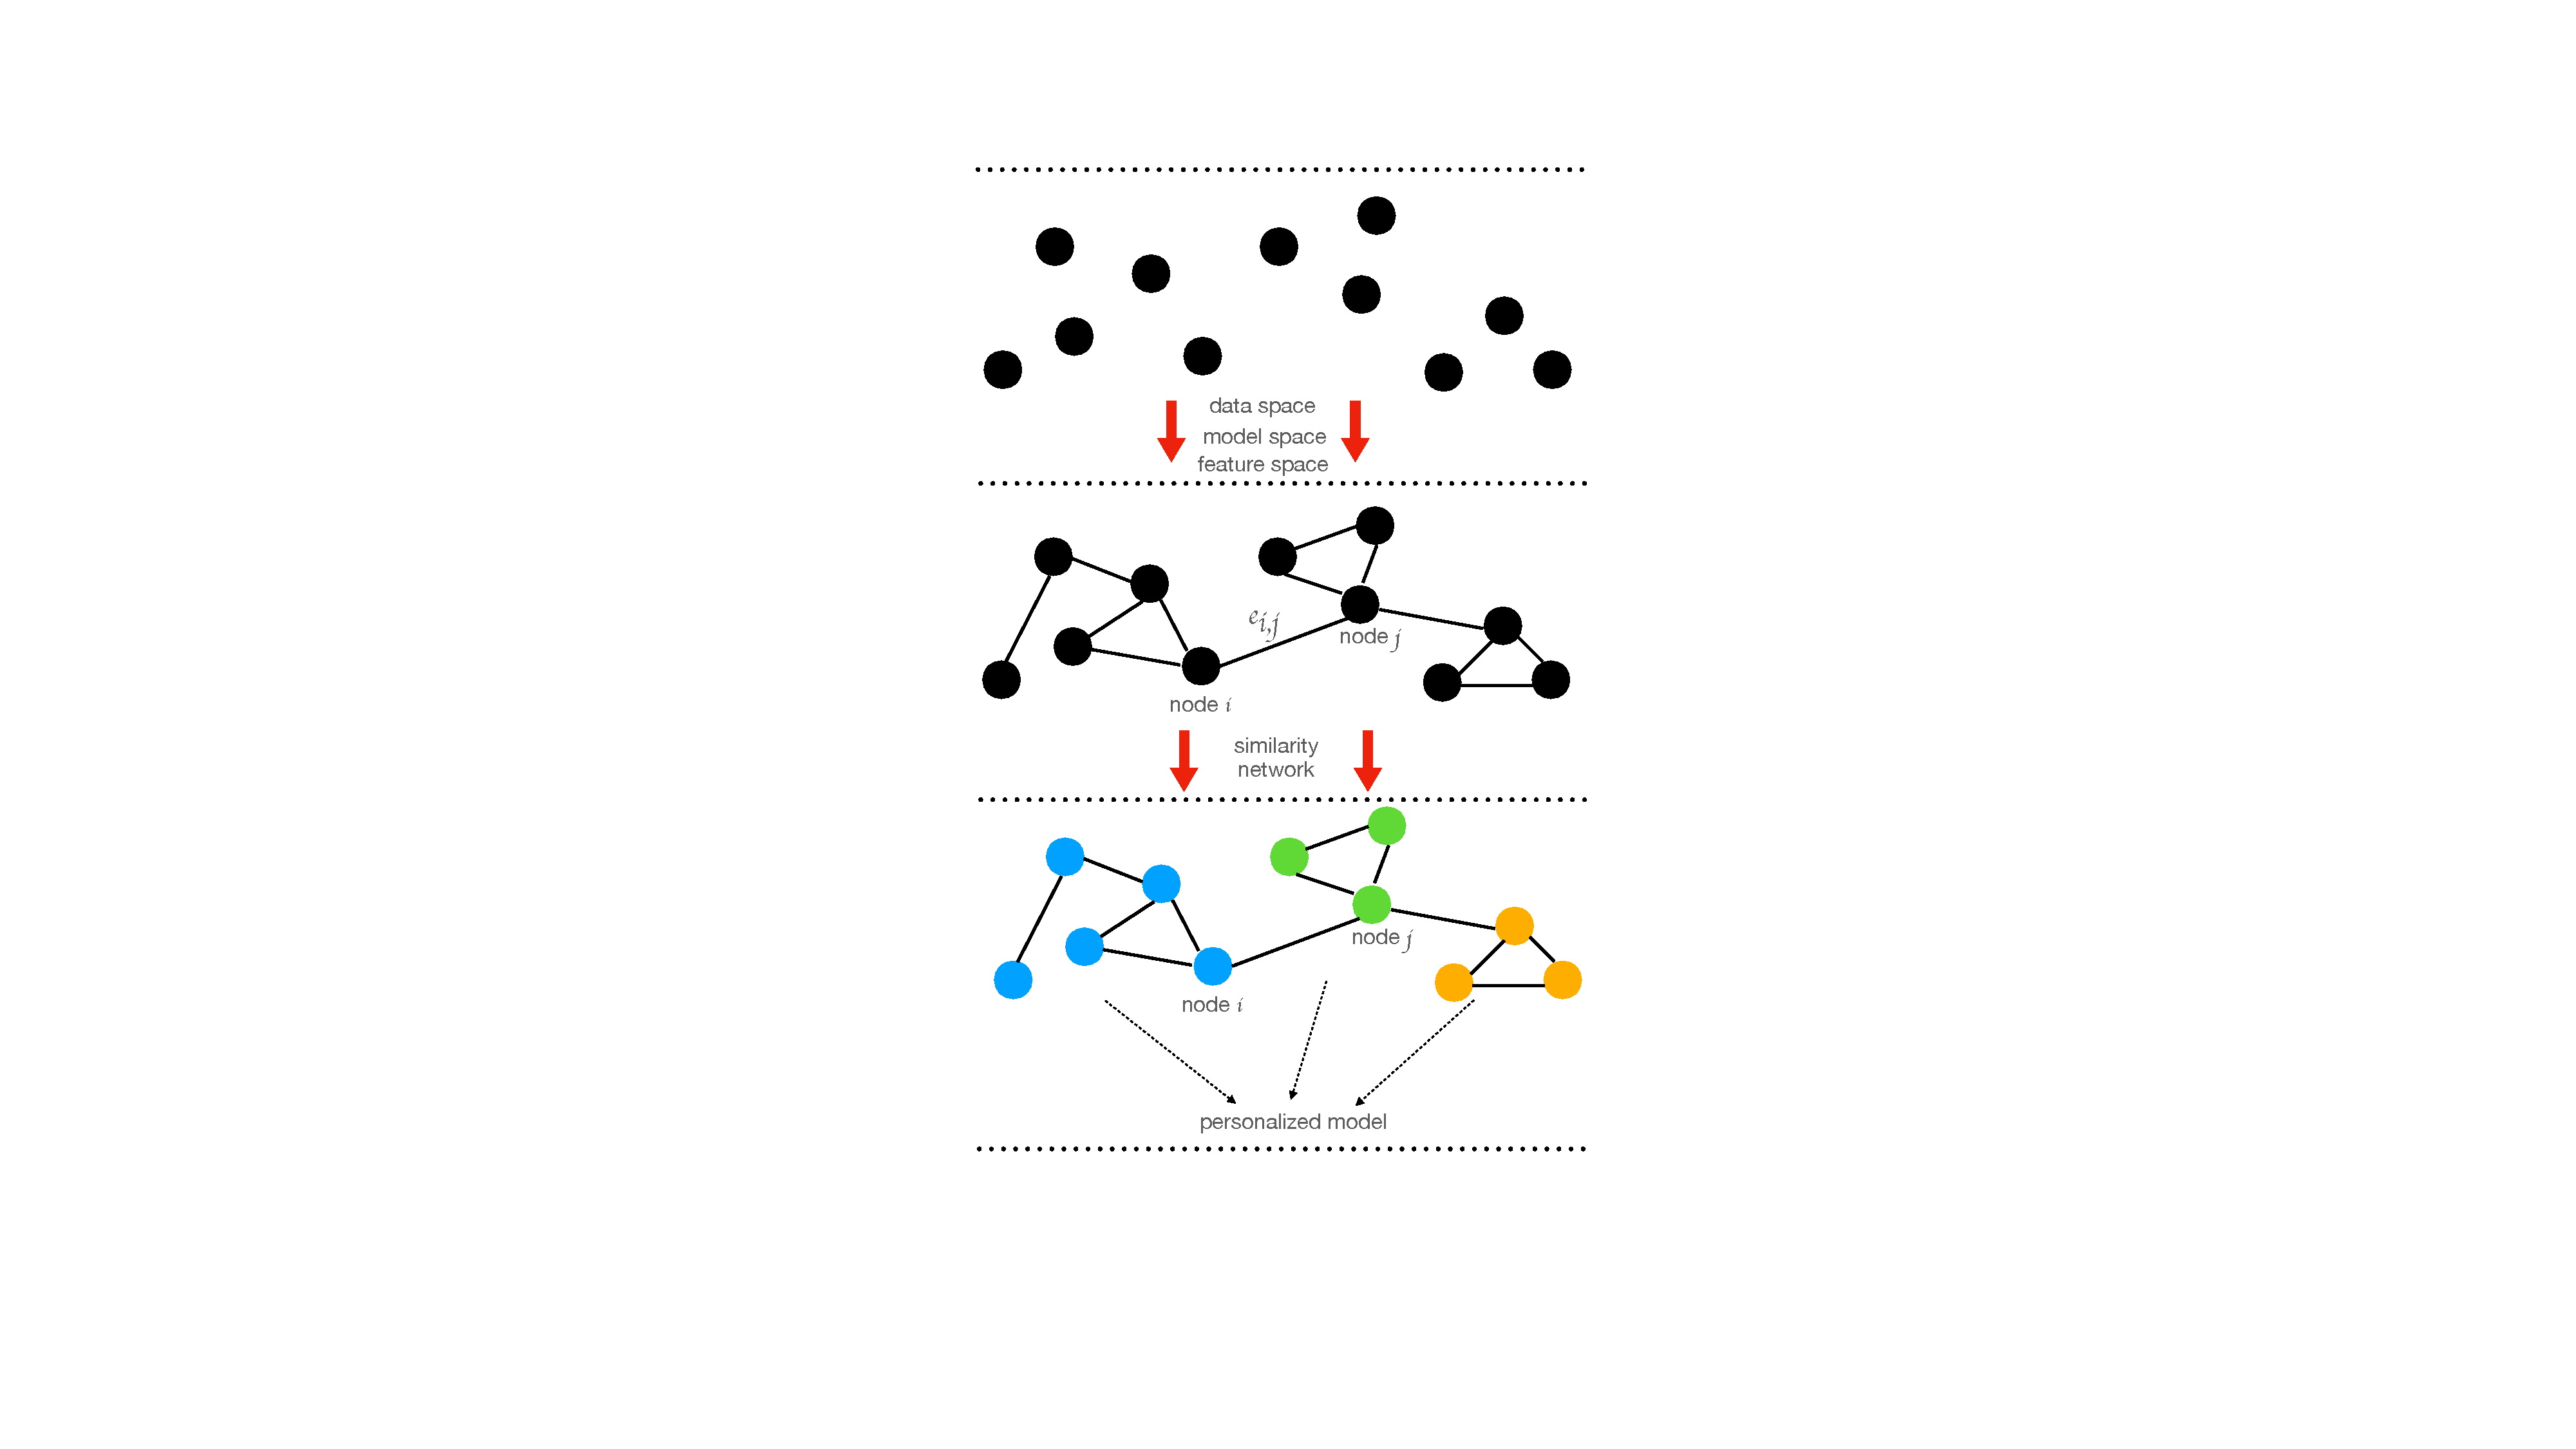
\includegraphics[width=0.97\columnwidth]{figs/figs_networkG}
\caption{Personalized representation based on similarity network}
\label{figure_xxx}
\end{figure}



\subsection{Final Formulation}
Given the mapping matrix $\M\in\RR^{d\times d_1}$ and $\N\in\RR^{d\times d_2}$, the objective problem is formulated by
\begin{align}
\min_{\substack{\{\x^{(n)}\}_{n=1}^N}} \sum_{n\in\Ncal} f_n\lrincir{\x^{(n)}; \A_n} + \lambda \sum_{\substack{e_{i,j} \in \Ecal,\\ \forall i,j\in\Ncal}} \lrnorm{\z^{(i)} - \z^{(j)}}_p,
\end{align} subject to:
\begin{align}
\x^{(n)} = \M\x + \N \z^{(n)},{~~~~}\forall n\in\Ncal, \x\in\RR^{d_1}, \z^{(n)}\in\RR^{d_2}.
\end{align} Here, $p\in\{1,2,\infty\}$. $\M$ and $\N$ has special structure, where every row of them has at most one non-zero value, and the non-zero value is $1$.  

The formulation equals to the following problem.
\begin{align}
\min_{\substack{\{\x^{(n)}\}_{n=1}^N}} \sum_{n\in\Ncal} f_n\lrincir{\x^{(n)}; \A_n} + \lambda \lrnorm{\z^{(i)} - \z^{(j)}}_p,
\end{align} subject to:
\begin{align}
\x^{(n)} = \M\x + \N \z^{(n)},{~~~~}\forall n\in\Ncal, \x\in\RR^{d_1}, \z^{(n)}\in\RR^{d_2}.
\end{align} 





\begin{figure}[!t]
\setlength{\abovecaptionskip}{0pt}
\setlength{\belowcaptionskip}{0pt}
\centering 
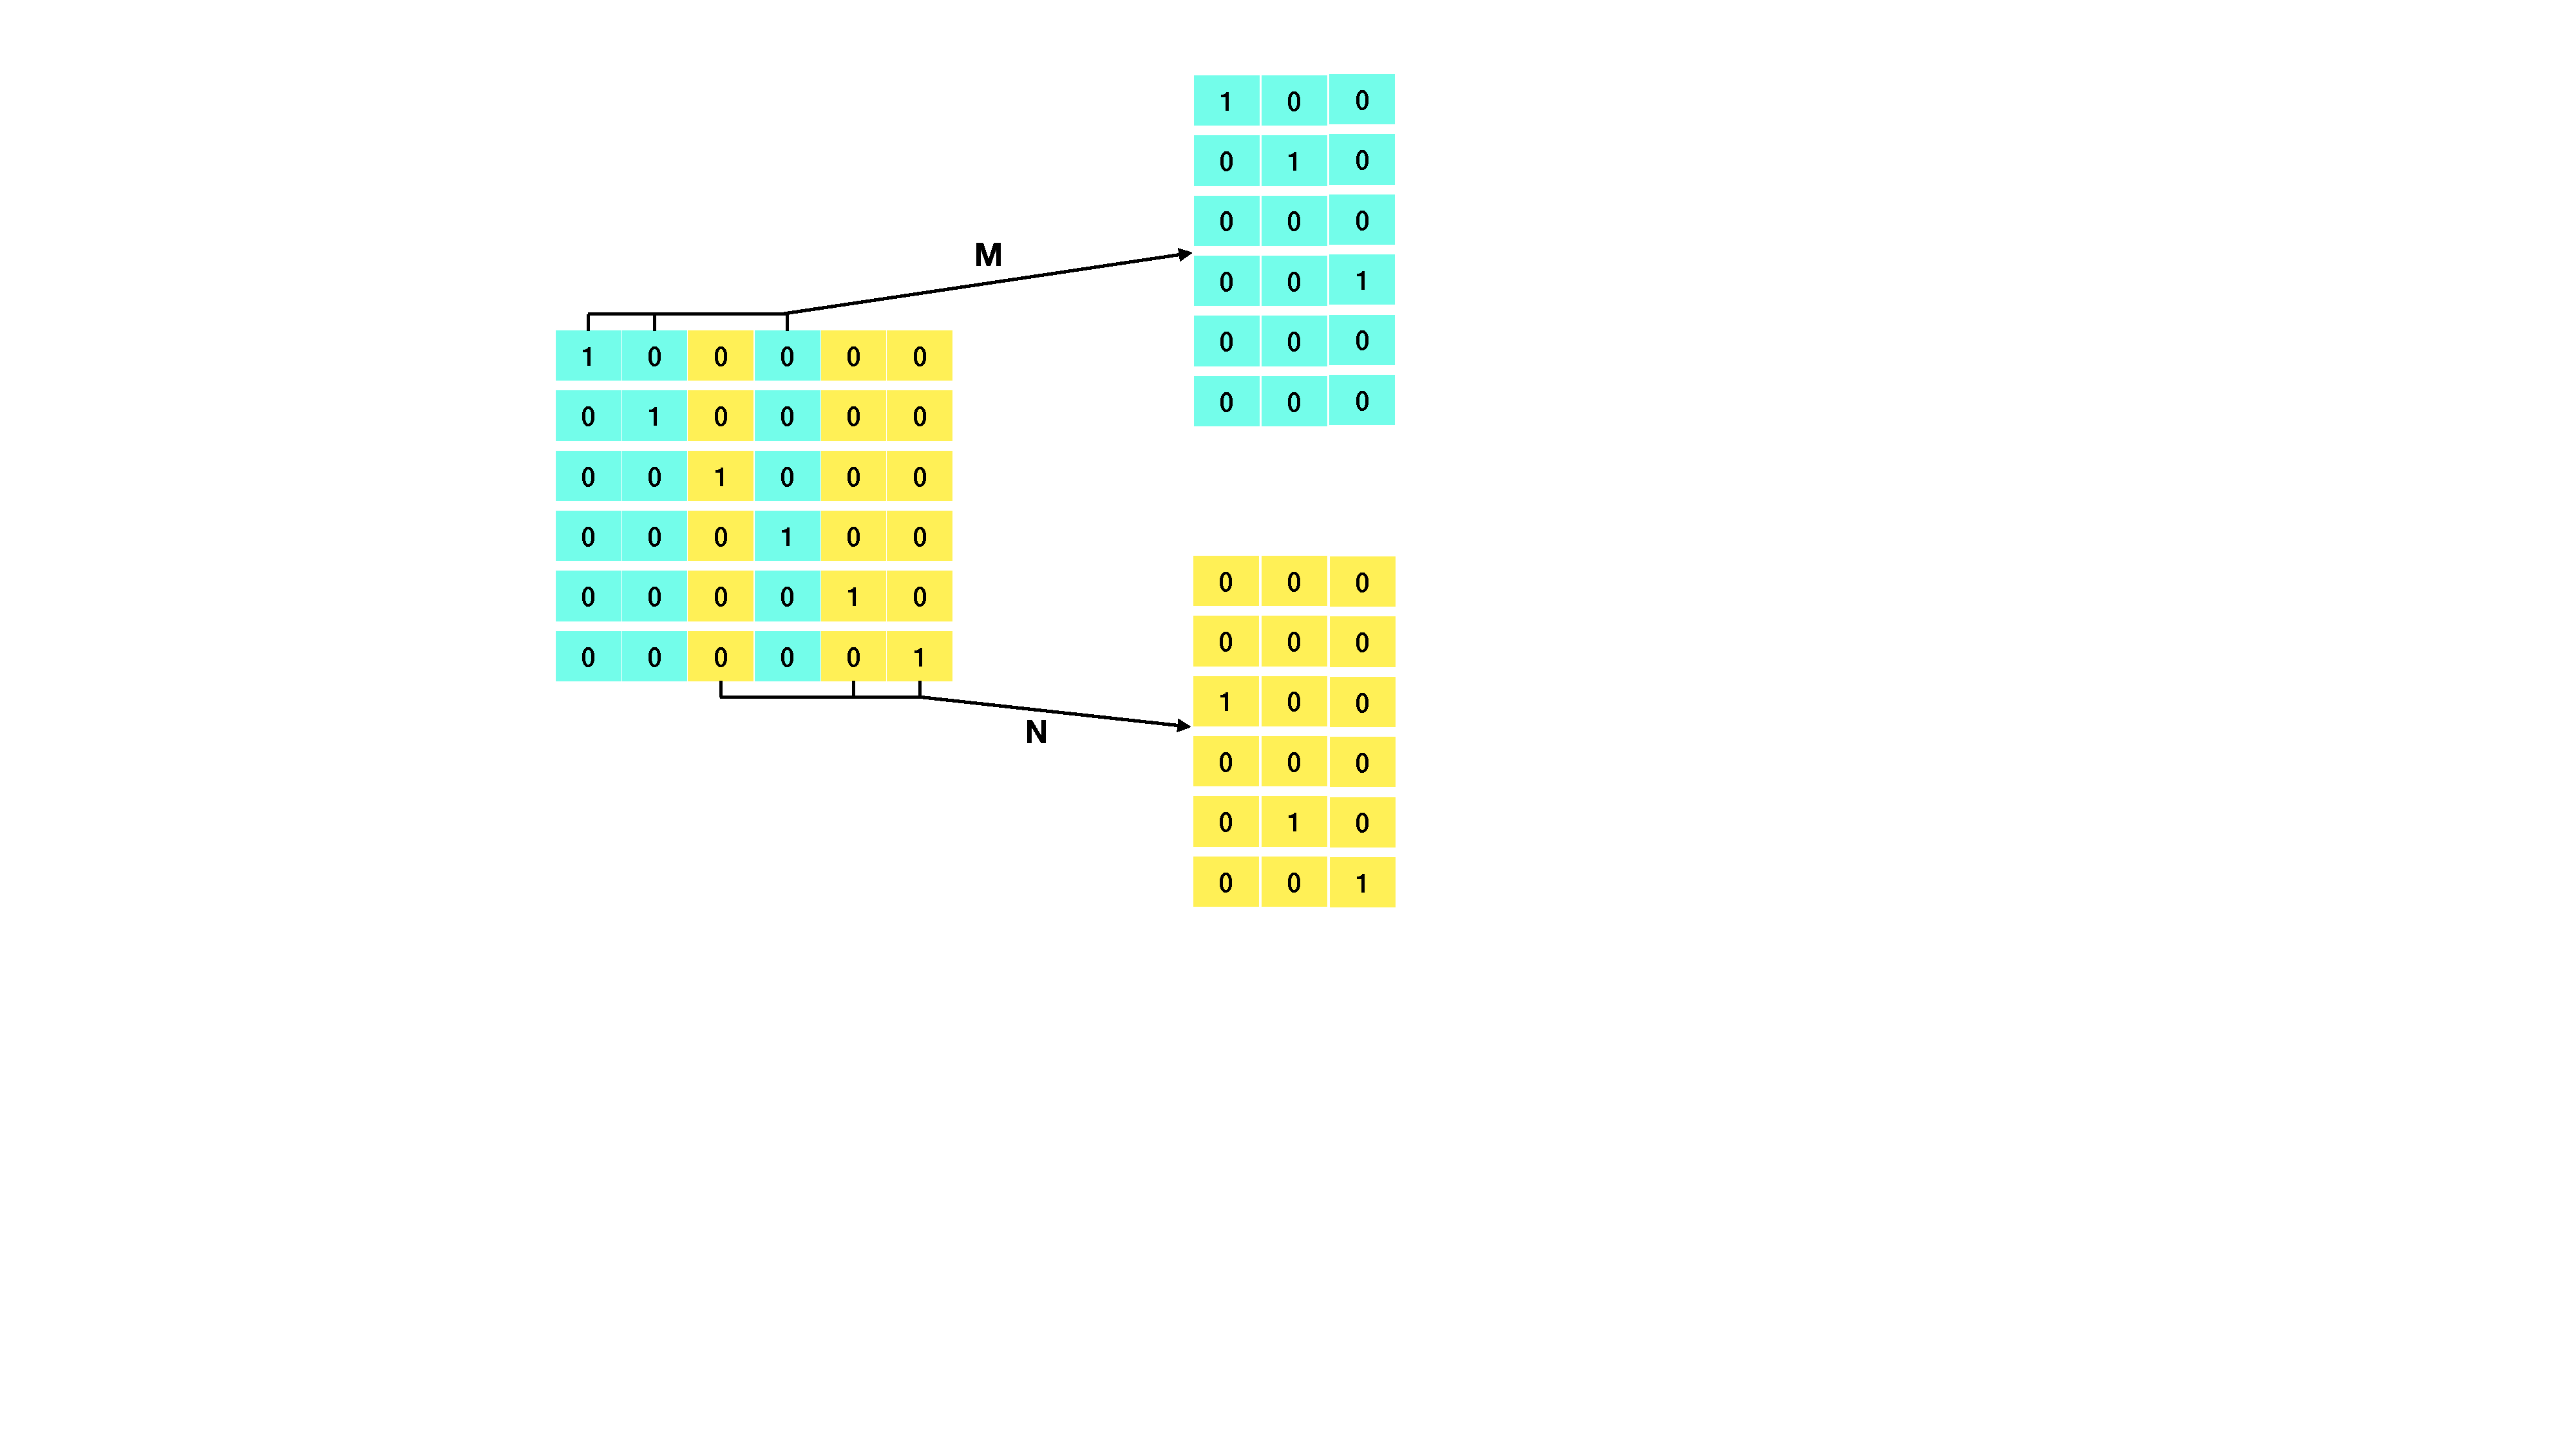
\includegraphics[width=0.97\columnwidth]{figs/figs_MNmatrix}
\caption{for example: $\M$ and $\N$ }
\label{figure_xxx}
\end{figure}




\subsection{Federated Optimization Methods}

The update of local model $\x^{(n)}_{t+1}$ is obtained by solving the following problem.
\begin{align}
\min_{\substack{\x^{(n)}\in\RR^{d}}} f_n\lrincir{\x^{(n)}; \A_n} + \lambda \sum_{\substack{e_{n,j} \in \Ecal,\\ \forall j\in\Ncal}} \lrnorm{\z^{(n)} - \z^{(j)}},
\end{align} subject to:
\begin{align}
\x^{(n)} = \M\x + \N \z^{(n)}.
\end{align} By using SGD \cite{xx}, the local model is updated by performing the following problem.
\begin{align}
\min_{\substack{\x^{(n)}\in\RR^{d}}} \lrangle{\g_t^{(n)}, \x^{(n)}-\x_t} + \lambda \sum_{\substack{e_{n,j} \in \Ecal,\\ \forall j\in\Ncal}} \lrnorm{\z^{(n)} - \z^{(j)}} + \frac{1}{2\eta}\lrnorm{\x^{(n)} - \x_t}^2,
\end{align} subject to:
\begin{align}
\x^{(n)} = \M\x + \N \z^{(n)}.
\end{align}








\textbf{On client.}  


\textbf{On server.}

\section{Communication Efficient Training}



\section{Empirical Studies}









\section*{Acknowledgment}
This work was supported by the xx. 



%\bibliographystyle{IEEEtran}  
%\bibliography{reference}


%\begin{IEEEbiography}[{\includegraphics[width=1in,height=1.25in,clip,keepaspectratio]{Yawei.pdf}}]{Yawei Zhao} is currently a Ph.D. candidate in Computer Science from the National University of Defense Technology, China. He received his B.E. degree and M.S. degree in Computer Science from the National University of Defense Technology, China, in 2013 and 2015, respectively. His research interests include asynchronous and parallel optimization algorithms, pattern recognition and machine learning.
%[{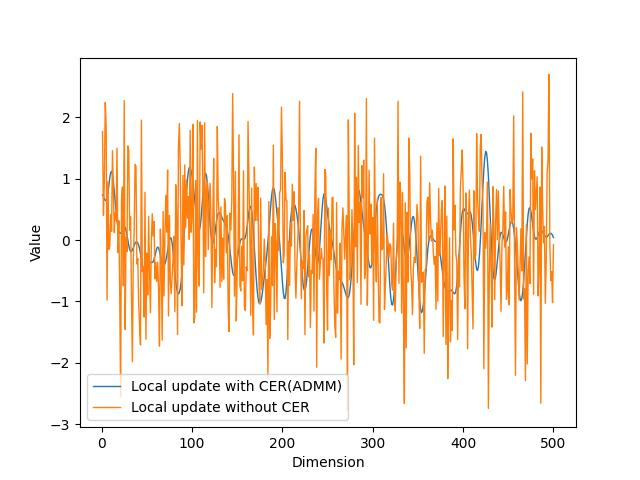
\includegraphics[width=1in,height=1.25in,clip,keepaspectratio]{xxx.pdf}}]{Yawei Zhao} is currently a Ph.D. candidate in Computer Science from the National University of Defense Technology, China. He received his B.E. degree and M.S. degree in Computer Science from the National University of Defense Technology, China, in 2013 and 2015, respectively. His research interests include asynchronous and parallel optimization algorithms, pattern recognition and machine learning.
%[{\includegraphics[width=1in,height=1.25in,clip,keepaspectratio]{jiliu.jpg}}]{Ji Liu} is currently a Ph.D. candidate in Computer Science from the National University of Defense Technology, China. He received his B.E. degree and M.S. degree in Computer Science from the National University of Defense Technology, China, in 2013 and 2015, respectively. His research interests include asynchronous and parallel optimization algorithms, pattern recognition and machine learning.
%\end{IEEEbiography}




\end{document}


